\chapter{相关理论与技术}\label{chap:theories_tech}

% \section{可观测性}

\section{BPF技术}

eBPF(Extended Berkeley Packet Filter)是Linux内核中的一个轻量级、快速的64位的类RISC虚拟机\citep{sharaf2022extended}。当前eBPF当前已经成为在Linux内核运行时执行不可信的、由用户定义的专用代码的最佳实践与事实标准。其强大的性能、可移植性、灵活性与安全性得到了工业界和学术界的认可,并被广泛地用于更多的领域。

eBPF的前身是BPF(Berkeley Packet Filter),最早由McCanne和Jacobson设计并提出\citep{mccanne1993bsd},起初BPF如其名称所示,用于在Linux网络子系统中对网络包进行灵活处理,而因其本身优异的设计,被Linux内核社区的贡献者扩展到内核的各个子系统中,来对内核功能进行定制化,为了与旧BPF技术进行区分,内核社区将早期的BPF技术成为cBPF(Classic Berkeley Packet Filter),而BPF和eBPF均指代最新的BPF技术,本文在后续说明中也采用这种做法。

BPF本身是一种指令集,最初设计时考虑到安全性与易用性,允许开发者使用C语言的子集进行编写,并能作为一种编译器后端指令集,由GCC等常用编译器编译为字节码\citep{ebpfguidence}。BPF采用字节码的处于两种原因,其一是方便内核验证器对代码进行验证,其二则与Java思想类似,即利用字节码与语言虚拟机的组合提升可移植性。BPF虚拟机运行在内核中,Linux提供了相关的BPF系统调用来将字节码加载到内核中,并附加到代码中声明的钩子函数处,当对应函数触发时,内核态的BPF虚拟机就会执行附加的BPF字节码。整个过程中为了防止加载非法代码,内核首先会在加载BPF代码前对BPF字节码进行验证,判断是否符合在内核中执行的规范,如不允许死循环等,而在内核BPF虚拟机中执行时,会利用JIT技术将字节码映射到本机机器码,从而实现最佳的运行性能。

同作为对内核功能的扩展,BPF技术经常会与内核模块进行比较。相较于内核模块,BPF技术具有更高的安全性,BPF程序安全性体现在三个方面。首先不同于内核模块,BPF程序在编写时所有的对内核数据、地址的访问都需要通过BPF Helper函数来实现,同时,部分BPF Helper函数设计时就考虑到并发性,极大减少了不安全代码的数量。其次,BPF代码在加载时会被内核验证,同时由于运行在虚拟机中,也增强了安全性。最后,BPF代码所能执行的位置由内核提供,这样也大大缩小了危险代码的影响范围。

\begin{figure}[!htbp]
    \centering
    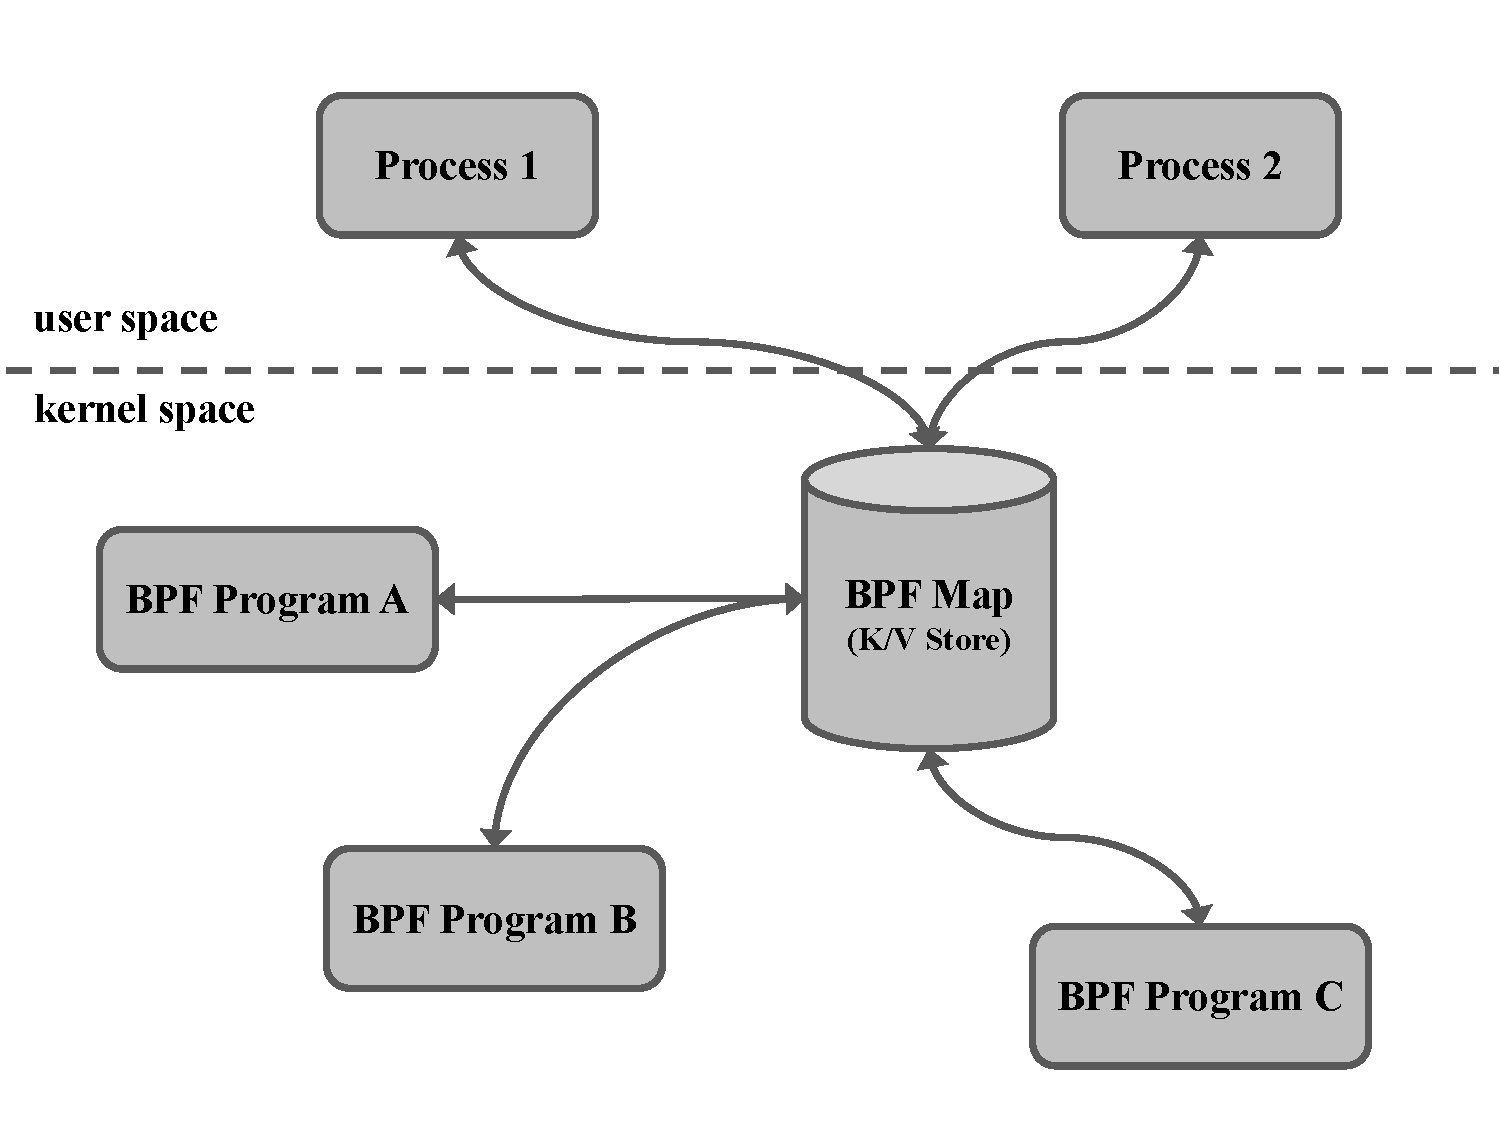
\includegraphics[width=0.6\textwidth]{bpf_user_kernel}
    \bicaption{\quad BPF中用户态与内核态的交互}{\quad Interaction between user mode and kernel mode in BPF}
    \label{fig:bpf_user_kernel}
\end{figure}

同时,BPF技术也具备高度的灵活性。这种灵活性体现在两个方面,首先对于用户态与内核态的交互,BPF技术运行由用户态的程序来加载BPF代码,由于BPF本身是字节码,因此能够借助libbpf等工具来对代码中的部分进行修改,这大大增强了BPF代码的灵活性。其次,如图~\ref{fig:bpf_user_kernel}所示,BPF技术允许通过BPF Map来实现用户态与内核的逻辑交互,一方面,内核态BPF程序所收集到的数据,能够借助BPF Map反馈给用户态程序进行处理,另一方面用户态程序也能通过BPF系统调用操作内BPF Map,对其中的内容进行读写,从而影响内核态BPF程序的行为。其次,BPF技术还允许BPF程序之间的交互,除上述通过BPF Map的交互外,如图~\ref{fig:bpf_to_bpf}所示,BPF程序还能够相互进行调用,从而进行数据传递,或通过多个BPF程序的调用,来突破内核对单个BPF函数的限制,从而实现更加复杂的代码逻辑。

\begin{figure}[!htbp]
    \centering
    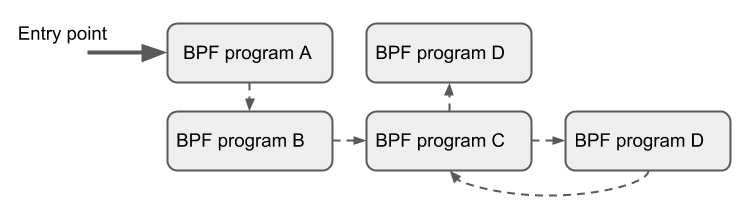
\includegraphics[width=0.7\textwidth]{bpf_to_bpf}
    \bicaption{\quad BPF程序之间的调用}{\quad Interaction between BPF programs}
    \label{fig:bpf_to_bpf}
\end{figure}

然而BPF技术也存在设计上的不足。由于在设计时首要考虑的是安全性,因此BPF程序在编写受到了种种限制,实际上,编写BPF程序所能使用的C语言子集是非图灵完备的,同时BPF程序在栈空间上也有严格的要求。这些限制都极大削弱了BPF程序的表达能力,使得其能够编写的逻辑十分有限。内核社区关注到这一点,并在近期的版本更新中逐步地减少对BPF程序的限制。

\section{Sched Ext}

Sched Ext是一种可扩展的内核调度器设计\citep{schedext},由Meta以及内核社区的工程师共同设计实现,并已经在Meta的集群中运行与测试。Sched Ext最早提出于2022年,当前尚未合并入内核主线,但Meta与内核社区开发者十分活跃,Sched Ext当前仍然正在积极更新并持续地向内核社区提交Patch。

Sched Ext启发自ghOSt\citep{humphries2021ghost},其同样考虑到内核调度器在开发与部署上的困难,与当前数据中心对于定制调度器的需求的不匹配,因此以设计一种插件化的调度器,来提升内核调度器开发的灵活性。然而不同于ghOSt,Sched Ext在设计初就尽可能地保持与Linux现有调度就机制的兼容性,这点在Sched Ext调度类的优先级上就有所体现,如图~\ref{fig:sched_ext_priorty}所示,开发者有意将Sched Ext调度类的优先级定义在Sched Normal之下,这就使得常规应用仍然可以由Sched Normal处理,从而最大地与当前Linux的调度机制兼容。

\begin{figure}[!htbp]
    \centering
    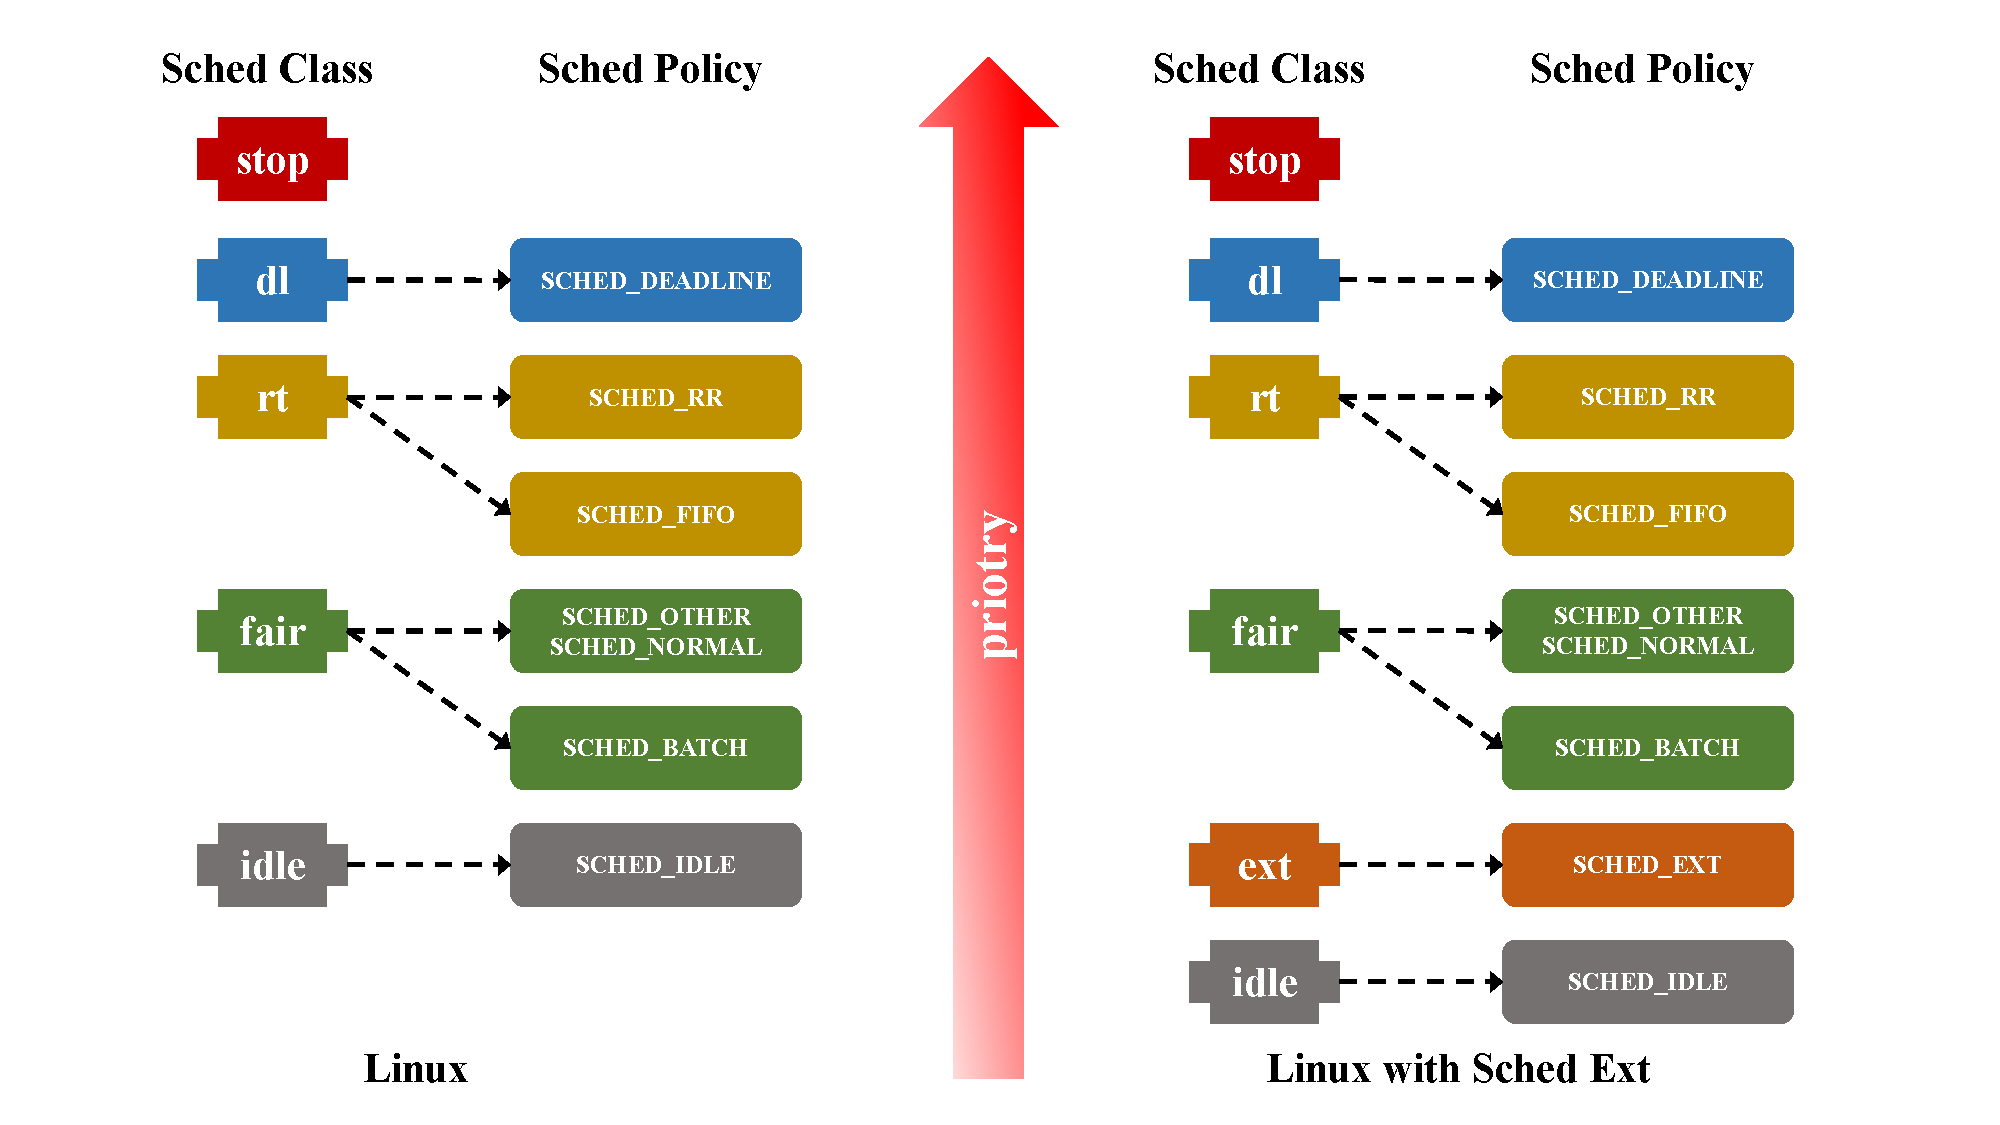
\includegraphics[width=1.0\textwidth]{sched_ext_priorty}
    \bicaption{\quad Sched Ext 调度优先级}{\quad Sched Ext Priorty}
    \label{fig:sched_ext_priorty}
\end{figure}

Sched Ext调度类实现了所有调度类方法,但是在每个方法的实现中,仅进行了函数开头的设置与结尾时资源的回收,所有调度相关的核心实现都依赖BPF函数中的实现:

1)enqueue\_task,当一个任务需要被加入到调度器的就绪队列时被调用,从而将进程加入到就绪队列,准备进行调度。

2)dequeue\_task,当一个任务不再需要调度(如被挂起或完成)时被调用,从就绪队列中移除进程。

3)yield\_task,当一个任务主动放弃CPU时间时,通常是在执行了yield系统调用后被调用,从而允许其他进程使用当前未使用的时间片。

4)check\_preempt\_curr,在每次任务唤醒时检查是否需要抢占当前运行的任务,从而确定当前运行的任务是否应该被新唤醒的任务抢占。

5)pick\_next\_task,选择下一个要运行的任务,一般从就绪队列中选择下一个要执行的任务。

6)put\_prev\_task,当前运行的任务停止运行时被调用,通常需要更新该任务的调度信息,并在其还有继续运行时放回就绪队列。

7)set\_curr\_task,每次切换到新任务时被调用,通常用于更新调度器的指示当前任务的curr指针。

8)task\_tick,每次系统时钟中断发生时被调用,一般时更新当前任务的调度信息,同时也包括当任务时间片使用完时执行抢占。

9)task\_fork,当一个新的任务被创建(fork)时被调用,通常用于处理新任务的调度相关设置。

10)task\_dead,当一个任务彻底结束并且要被移除时被调用,用于清理该任务的调度相关资源。


\begin{figure}[!htbp]
    \centering
    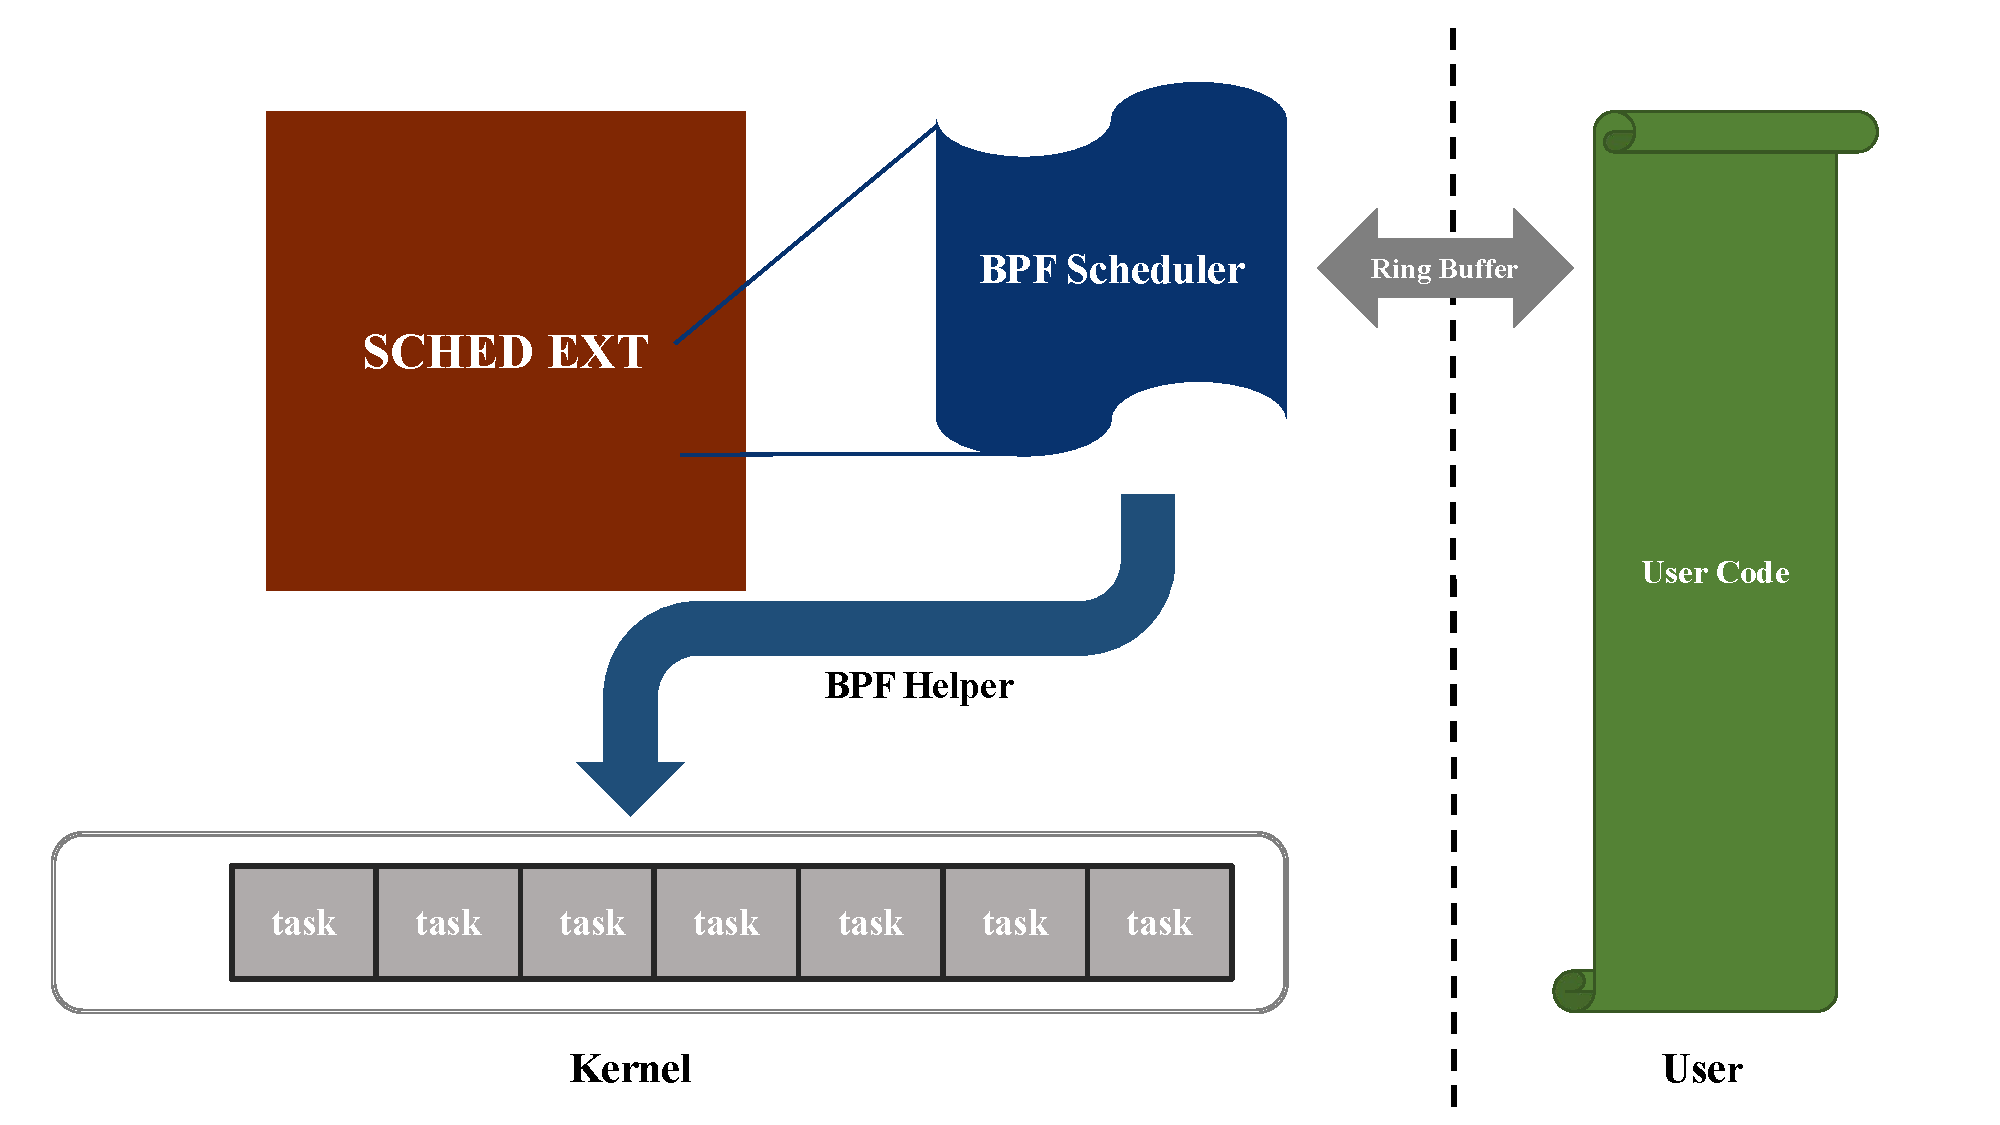
\includegraphics[width=0.7\textwidth]{sched_ext_arch}
    \bicaption{\quad Sched Ext架构}{\quad Sched Ext Arch}
    \label{fig:sched_ext_arch}
\end{figure}

如图~\ref{fig:sched_ext_arch}所示,Sched Ext基于BPF的可编程设计提供了丰富的手段来定制化调度过程。首先最直接的就是通过BPF代码定制调度逻辑,,这种方式的好处就在于所有的调度过程仍然在内核中进行,因此不会有用户态与内核态频繁切换的开销,而开发者仅需要提交BPF代码。其次,开发者可以直接操作任务队列来控制调度过程,Sched Ext将调度中核心的任务队列暴漏了出来,并允许通过BPF Help函数直接操作任务队列,这使得在调度程序完全能够在用户态进行实现,同时Sched Ext还提供了基于C与Rust语言的库函数,方便了开发者进行调度器设计,这种方式虽然引入了地址空间切换的开销,但也极大增加了调度器设计的灵活性。

默认情况下仅由Sched Ext类的任务会被BPF调度程序处理,而如果BPF调度程序尚未加载,Sched Ext调度类的任务仍然会交给Sched Normal进行处理,以避免任务得不到执行。同时,Sched Ext还允许通过特殊的BPF Helper函数,将SCHED NORMAL即以下的任务全部交给SCHED EXT进行处理,这种情况下,Sched Ext调度类就能够参与系统中核心的调度过程。

% \section{沙箱技术}

% % 系统级沙箱(虚拟机),容器级沙箱(进程)

% 沙箱技术是一种安全机制,用于隔离运行环境,以便在受限的环境中执行不受信任的程序或代码,并防止这些程序或代码对主机上其他任务造成影响或危害。沙箱是通过在受限的操作系统环境中执行软件来实现的,并对软件所能使用的资源,如CPU、内存、网络等进行限制。沙箱技术为在数据中心中安全地运行各种各样的应用提供了基础,而在数据中心中,常见的沙箱技术包括虚拟机技术与容器技术。

% 虚拟机技术是数据中心应用最广泛的沙箱技术,通常指通过软硬件的手段,在已运行的系统中模拟出一个硬件环境,并能够支持运行其他系统。虚拟机技术最早提出于\citep{bugnion1997disco}, 用于解决操作系统迭代速度与硬件更新速度不匹配的问题,而后

\section{本章小结}

本章主要介绍了eBPF技术以及Sched Ext可扩展内核调度机制。其中eBPF技术提供了一种集性能、灵活性于安全性于一体的扩展内核方式,利用eBPF技术能够方便地从内核中获取更多细致的数据,同时也能够在一些支持相对丰富的内核子系统中对内核功能进行定制。而Sched Ext提供了一种内核主线之外扩展内核调度的方式,其本身基于eBPF技术,因而能够利用到eBPF本身所具备的优势,同时其在调度子系统中展开了许多工作,使得通过eBPF程序定制调度逻辑成为可能,而其在设计上对于兼容性的考量,也方便了其在生产环境中的部署于测试。如上技术为本论文对应用进行细粒度监控,构造Control Zone与为不同混部场景设计不同的调度策略奠定了基础。